\section{Introduction}
\label{sec:intro}

\begin{figure*}[t]
  \centering
  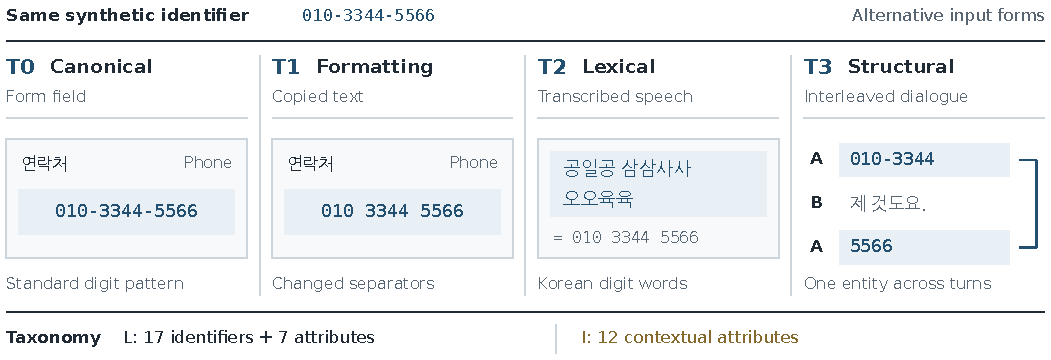
\includegraphics[width=\textwidth]{figures/fig1_overview.pdf}
  \caption{\textbf{One identifier, four input forms in \kiii{}.}
  A synthetic phone number appears in canonical (T0), formatting (T1), lexical
  (T2), and structural (T3) forms. Shading marks identifier spans; the bracket
  links speaker A's fragments across B's interruption (``mine too'').
  Examples are illustrative, not paired corpus records. The footer summarizes
  the Legal (L) and Identifiability (I) tiers.}
  \Description{Four aligned panels show the synthetic phone number
  010-3344-5566 with hyphens, with spaces, as Korean digit words, and split into
  010-3344 and 5566 across two turns by speaker A, interrupted by speaker B.
  A bracket links the two fragments. The footer summarizes 17 Legal identifiers,
  7 Legal attributes, and 12 Identifiability attributes.}
  \label{fig:overview}
\end{figure*}


%% Paragraph 1: the DLP problem. Regex solves canonical PII; real text is not canonical.
Korean financial institutions are required to prevent personal (credit) information from leaving controlled systems, and increasingly deploy LLM-based DLP filters on unstructured text. For canonical strings---a resident registration number written \texttt{900101-1234567}, a card number with a valid Luhn digit---a regular expression with a checksum is near-perfect. The difficulty is everywhere else: a customer dictating an account number as \emph{일일공 에 일이삼 에 사오육칠팔구} over the phone, a number split across two turns and read back by the agent, a scanned statement whose zeros became the letter O, a ``masked'' RRN that still exposes birth date and sex. \todo{one sentence with a concrete leakage anecdote or statistic if available}

%% Paragraph 2: why existing benchmarks do not measure this.
Existing PII benchmarks do not measure this. English benchmarks~\cite{shen2025piibench,vats2026redact} lack Korean; the only Korean PII resources are conversational~\cite{fei2024kdpii,jang2024koreanpiiner} or legal~\cite{hahm2025thunderdeid}, define categories without statutory grounding, and present identifiers in canonical form. None models how Korean speech-to-text output renders numbers, although call-centre transcripts are the largest unstructured PII stream in the sector.

%% Paragraph 3: contributions (4 bullets max).
Figure~\ref{fig:overview} illustrates the controlled input variations and taxonomy
underlying \kiii{}. We make three contributions.
\begin{enumerate}
  \item A \textbf{regulation-grounded, two-tier taxonomy} of 36 categories: 24 \emph{Legal} categories each cited to a statutory article (\S\ref{sec:taxonomy}), and 12 \emph{Identifiability} categories capturing quasi-identifiers and behavioural attributes that enable profiling.
  \item A \textbf{synthetic long-context, multi-subject corpus} in which identifiers are generated by code (checksum-valid) and rendered through a controlled \textbf{surface-form variation} axis (T0--T3) calibrated to Korean STT behaviour (\S\ref{sec:benchmark}).
  \item A \textbf{leaderboard} of \todo{N} systems spanning rule baselines, frontier APIs, open-weight and Korean-developed LLMs, with analysis by tier, variation level, subject count and context length (\S\ref{sec:results}).
\end{enumerate}
